% Created by tikzDevice version 0.12.3 on 2020-05-26 21:47:23
% !TEX encoding = UTF-8 Unicode
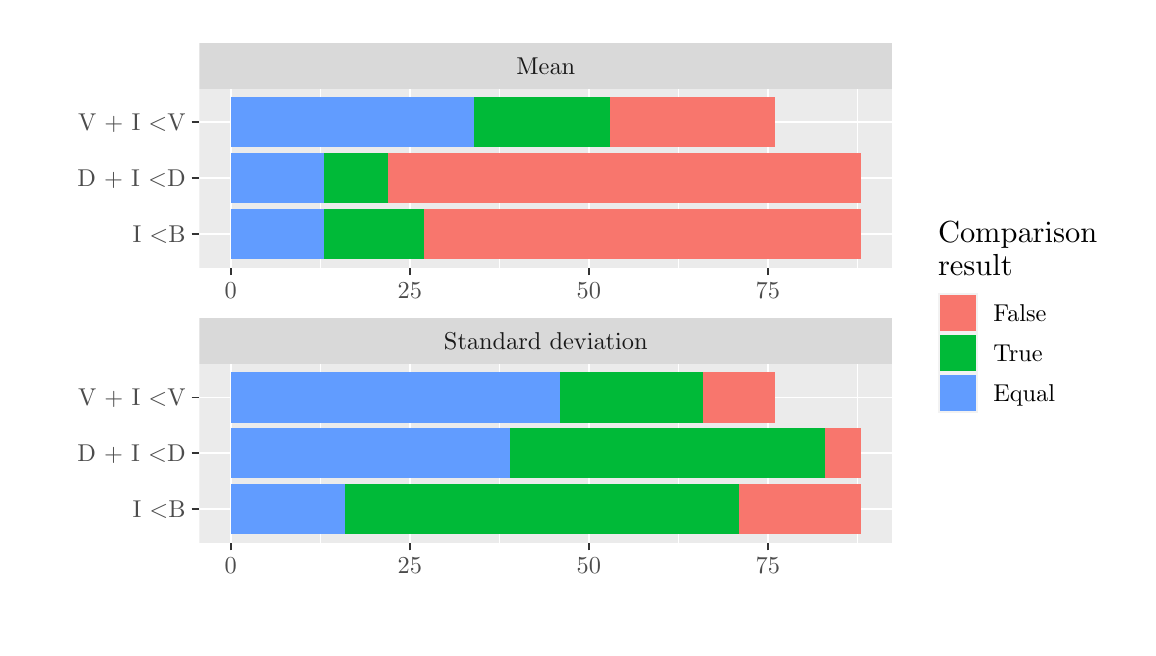
\begin{tikzpicture}[x=1pt,y=1pt]
\definecolor{fillColor}{RGB}{255,255,255}
\path[use as bounding box,fill=fillColor,fill opacity=0.00] (0,0) rectangle (397.48,216.81);
\begin{scope}
\path[clip] (  0.00,  0.00) rectangle (397.48,216.81);
\definecolor{drawColor}{RGB}{255,255,255}
\definecolor{fillColor}{RGB}{255,255,255}

\path[draw=drawColor,line width= 0.6pt,line join=round,line cap=round,fill=fillColor] (  0.00,  0.00) rectangle (397.48,216.81);
\end{scope}
\begin{scope}
\path[clip] ( 62.02,130.11) rectangle (312.46,194.74);
\definecolor{fillColor}{gray}{0.92}

\path[fill=fillColor] ( 62.02,130.11) rectangle (312.46,194.74);
\definecolor{drawColor}{RGB}{255,255,255}

\path[draw=drawColor,line width= 0.3pt,line join=round] (105.74,130.11) --
	(105.74,194.74);

\path[draw=drawColor,line width= 0.3pt,line join=round] (170.42,130.11) --
	(170.42,194.74);

\path[draw=drawColor,line width= 0.3pt,line join=round] (235.10,130.11) --
	(235.10,194.74);

\path[draw=drawColor,line width= 0.3pt,line join=round] (299.79,130.11) --
	(299.79,194.74);

\path[draw=drawColor,line width= 0.6pt,line join=round] ( 62.02,142.23) --
	(312.46,142.23);

\path[draw=drawColor,line width= 0.6pt,line join=round] ( 62.02,162.42) --
	(312.46,162.42);

\path[draw=drawColor,line width= 0.6pt,line join=round] ( 62.02,182.62) --
	(312.46,182.62);

\path[draw=drawColor,line width= 0.6pt,line join=round] ( 73.40,130.11) --
	( 73.40,194.74);

\path[draw=drawColor,line width= 0.6pt,line join=round] (138.08,130.11) --
	(138.08,194.74);

\path[draw=drawColor,line width= 0.6pt,line join=round] (202.76,130.11) --
	(202.76,194.74);

\path[draw=drawColor,line width= 0.6pt,line join=round] (267.44,130.11) --
	(267.44,194.74);
\definecolor{fillColor}{RGB}{248,118,109}

\path[fill=fillColor] (143.26,133.14) rectangle (301.08,151.32);
\definecolor{fillColor}{RGB}{0,186,56}

\path[fill=fillColor] (107.03,133.14) rectangle (143.26,151.32);
\definecolor{fillColor}{RGB}{97,156,255}

\path[fill=fillColor] ( 73.40,133.14) rectangle (107.03,151.32);
\definecolor{fillColor}{RGB}{248,118,109}

\path[fill=fillColor] (130.32,153.34) rectangle (301.08,171.51);
\definecolor{fillColor}{RGB}{0,186,56}

\path[fill=fillColor] (107.03,153.34) rectangle (130.32,171.51);
\definecolor{fillColor}{RGB}{97,156,255}

\path[fill=fillColor] ( 73.40,153.34) rectangle (107.03,171.51);
\definecolor{fillColor}{RGB}{248,118,109}

\path[fill=fillColor] (210.52,173.53) rectangle (270.03,191.71);
\definecolor{fillColor}{RGB}{0,186,56}

\path[fill=fillColor] (161.37,173.53) rectangle (210.52,191.71);
\definecolor{fillColor}{RGB}{97,156,255}

\path[fill=fillColor] ( 73.40,173.53) rectangle (161.37,191.71);
\end{scope}
\begin{scope}
\path[clip] ( 62.02, 30.69) rectangle (312.46, 95.32);
\definecolor{fillColor}{gray}{0.92}

\path[fill=fillColor] ( 62.02, 30.69) rectangle (312.46, 95.32);
\definecolor{drawColor}{RGB}{255,255,255}

\path[draw=drawColor,line width= 0.3pt,line join=round] (105.74, 30.69) --
	(105.74, 95.32);

\path[draw=drawColor,line width= 0.3pt,line join=round] (170.42, 30.69) --
	(170.42, 95.32);

\path[draw=drawColor,line width= 0.3pt,line join=round] (235.10, 30.69) --
	(235.10, 95.32);

\path[draw=drawColor,line width= 0.3pt,line join=round] (299.79, 30.69) --
	(299.79, 95.32);

\path[draw=drawColor,line width= 0.6pt,line join=round] ( 62.02, 42.80) --
	(312.46, 42.80);

\path[draw=drawColor,line width= 0.6pt,line join=round] ( 62.02, 63.00) --
	(312.46, 63.00);

\path[draw=drawColor,line width= 0.6pt,line join=round] ( 62.02, 83.20) --
	(312.46, 83.20);

\path[draw=drawColor,line width= 0.6pt,line join=round] ( 73.40, 30.69) --
	( 73.40, 95.32);

\path[draw=drawColor,line width= 0.6pt,line join=round] (138.08, 30.69) --
	(138.08, 95.32);

\path[draw=drawColor,line width= 0.6pt,line join=round] (202.76, 30.69) --
	(202.76, 95.32);

\path[draw=drawColor,line width= 0.6pt,line join=round] (267.44, 30.69) --
	(267.44, 95.32);
\definecolor{fillColor}{RGB}{248,118,109}

\path[fill=fillColor] (257.10, 33.72) rectangle (301.08, 51.89);
\definecolor{fillColor}{RGB}{0,186,56}

\path[fill=fillColor] (114.80, 33.72) rectangle (257.10, 51.89);
\definecolor{fillColor}{RGB}{97,156,255}

\path[fill=fillColor] ( 73.40, 33.72) rectangle (114.80, 51.89);
\definecolor{fillColor}{RGB}{248,118,109}

\path[fill=fillColor] (288.14, 53.91) rectangle (301.08, 72.09);
\definecolor{fillColor}{RGB}{0,186,56}

\path[fill=fillColor] (174.30, 53.91) rectangle (288.14, 72.09);
\definecolor{fillColor}{RGB}{97,156,255}

\path[fill=fillColor] ( 73.40, 53.91) rectangle (174.30, 72.09);
\definecolor{fillColor}{RGB}{248,118,109}

\path[fill=fillColor] (244.16, 74.11) rectangle (270.03, 92.29);
\definecolor{fillColor}{RGB}{0,186,56}

\path[fill=fillColor] (192.41, 74.11) rectangle (244.16, 92.29);
\definecolor{fillColor}{RGB}{97,156,255}

\path[fill=fillColor] ( 73.40, 74.11) rectangle (192.41, 92.29);
\end{scope}
\begin{scope}
\path[clip] ( 62.02, 95.32) rectangle (312.46,111.89);
\definecolor{fillColor}{gray}{0.85}

\path[fill=fillColor] ( 62.02, 95.32) rectangle (312.46,111.89);
\definecolor{drawColor}{gray}{0.10}

\node[text=drawColor,anchor=base,inner sep=0pt, outer sep=0pt, scale=  0.88] at (187.24,100.57) {Standard deviation};
\end{scope}
\begin{scope}
\path[clip] ( 62.02,194.74) rectangle (312.46,211.31);
\definecolor{fillColor}{gray}{0.85}

\path[fill=fillColor] ( 62.02,194.74) rectangle (312.46,211.31);
\definecolor{drawColor}{gray}{0.10}

\node[text=drawColor,anchor=base,inner sep=0pt, outer sep=0pt, scale=  0.88] at (187.24,199.99) {Mean};
\end{scope}
\begin{scope}
\path[clip] (  0.00,  0.00) rectangle (397.48,216.81);
\definecolor{drawColor}{gray}{0.20}

\path[draw=drawColor,line width= 0.6pt,line join=round] ( 73.40, 27.94) --
	( 73.40, 30.69);

\path[draw=drawColor,line width= 0.6pt,line join=round] (138.08, 27.94) --
	(138.08, 30.69);

\path[draw=drawColor,line width= 0.6pt,line join=round] (202.76, 27.94) --
	(202.76, 30.69);

\path[draw=drawColor,line width= 0.6pt,line join=round] (267.44, 27.94) --
	(267.44, 30.69);
\end{scope}
\begin{scope}
\path[clip] (  0.00,  0.00) rectangle (397.48,216.81);
\definecolor{drawColor}{gray}{0.30}

\node[text=drawColor,anchor=base,inner sep=0pt, outer sep=0pt, scale=  0.88] at ( 73.40, 19.68) {0};

\node[text=drawColor,anchor=base,inner sep=0pt, outer sep=0pt, scale=  0.88] at (138.08, 19.68) {25};

\node[text=drawColor,anchor=base,inner sep=0pt, outer sep=0pt, scale=  0.88] at (202.76, 19.68) {50};

\node[text=drawColor,anchor=base,inner sep=0pt, outer sep=0pt, scale=  0.88] at (267.44, 19.68) {75};
\end{scope}
\begin{scope}
\path[clip] (  0.00,  0.00) rectangle (397.48,216.81);
\definecolor{drawColor}{gray}{0.20}

\path[draw=drawColor,line width= 0.6pt,line join=round] ( 73.40,127.36) --
	( 73.40,130.11);

\path[draw=drawColor,line width= 0.6pt,line join=round] (138.08,127.36) --
	(138.08,130.11);

\path[draw=drawColor,line width= 0.6pt,line join=round] (202.76,127.36) --
	(202.76,130.11);

\path[draw=drawColor,line width= 0.6pt,line join=round] (267.44,127.36) --
	(267.44,130.11);
\end{scope}
\begin{scope}
\path[clip] (  0.00,  0.00) rectangle (397.48,216.81);
\definecolor{drawColor}{gray}{0.30}

\node[text=drawColor,anchor=base,inner sep=0pt, outer sep=0pt, scale=  0.88] at ( 73.40,119.10) {0};

\node[text=drawColor,anchor=base,inner sep=0pt, outer sep=0pt, scale=  0.88] at (138.08,119.10) {25};

\node[text=drawColor,anchor=base,inner sep=0pt, outer sep=0pt, scale=  0.88] at (202.76,119.10) {50};

\node[text=drawColor,anchor=base,inner sep=0pt, outer sep=0pt, scale=  0.88] at (267.44,119.10) {75};
\end{scope}
\begin{scope}
\path[clip] (  0.00,  0.00) rectangle (397.48,216.81);
\definecolor{drawColor}{gray}{0.30}

\node[text=drawColor,anchor=base east,inner sep=0pt, outer sep=0pt, scale=  0.88] at ( 57.07,139.20) {I \textless B};

\node[text=drawColor,anchor=base east,inner sep=0pt, outer sep=0pt, scale=  0.88] at ( 57.07,159.39) {D + I \textless D};

\node[text=drawColor,anchor=base east,inner sep=0pt, outer sep=0pt, scale=  0.88] at ( 57.07,179.59) {V + I \textless V};
\end{scope}
\begin{scope}
\path[clip] (  0.00,  0.00) rectangle (397.48,216.81);
\definecolor{drawColor}{gray}{0.20}

\path[draw=drawColor,line width= 0.6pt,line join=round] ( 59.27,142.23) --
	( 62.02,142.23);

\path[draw=drawColor,line width= 0.6pt,line join=round] ( 59.27,162.42) --
	( 62.02,162.42);

\path[draw=drawColor,line width= 0.6pt,line join=round] ( 59.27,182.62) --
	( 62.02,182.62);
\end{scope}
\begin{scope}
\path[clip] (  0.00,  0.00) rectangle (397.48,216.81);
\definecolor{drawColor}{gray}{0.30}

\node[text=drawColor,anchor=base east,inner sep=0pt, outer sep=0pt, scale=  0.88] at ( 57.07, 39.77) {I \textless B};

\node[text=drawColor,anchor=base east,inner sep=0pt, outer sep=0pt, scale=  0.88] at ( 57.07, 59.97) {D + I \textless D};

\node[text=drawColor,anchor=base east,inner sep=0pt, outer sep=0pt, scale=  0.88] at ( 57.07, 80.17) {V + I \textless V};
\end{scope}
\begin{scope}
\path[clip] (  0.00,  0.00) rectangle (397.48,216.81);
\definecolor{drawColor}{gray}{0.20}

\path[draw=drawColor,line width= 0.6pt,line join=round] ( 59.27, 42.80) --
	( 62.02, 42.80);

\path[draw=drawColor,line width= 0.6pt,line join=round] ( 59.27, 63.00) --
	( 62.02, 63.00);

\path[draw=drawColor,line width= 0.6pt,line join=round] ( 59.27, 83.20) --
	( 62.02, 83.20);
\end{scope}
\begin{scope}
\path[clip] (  0.00,  0.00) rectangle (397.48,216.81);
\definecolor{fillColor}{RGB}{255,255,255}

\path[fill=fillColor] (323.46, 71.98) rectangle (391.98,153.44);
\end{scope}
\begin{scope}
\path[clip] (  0.00,  0.00) rectangle (397.48,216.81);
\definecolor{drawColor}{RGB}{0,0,0}

\node[text=drawColor,anchor=base west,inner sep=0pt, outer sep=0pt, scale=  1.10] at (328.96,139.30) {Comparison};

\node[text=drawColor,anchor=base west,inner sep=0pt, outer sep=0pt, scale=  1.10] at (328.96,127.42) {result};
\end{scope}
\begin{scope}
\path[clip] (  0.00,  0.00) rectangle (397.48,216.81);
\definecolor{fillColor}{gray}{0.95}

\path[fill=fillColor] (328.96,106.39) rectangle (343.42,120.85);
\end{scope}
\begin{scope}
\path[clip] (  0.00,  0.00) rectangle (397.48,216.81);
\definecolor{fillColor}{RGB}{248,118,109}

\path[fill=fillColor] (329.67,107.10) rectangle (342.71,120.13);
\end{scope}
\begin{scope}
\path[clip] (  0.00,  0.00) rectangle (397.48,216.81);
\definecolor{fillColor}{gray}{0.95}

\path[fill=fillColor] (328.96, 91.94) rectangle (343.42,106.39);
\end{scope}
\begin{scope}
\path[clip] (  0.00,  0.00) rectangle (397.48,216.81);
\definecolor{fillColor}{RGB}{0,186,56}

\path[fill=fillColor] (329.67, 92.65) rectangle (342.71,105.68);
\end{scope}
\begin{scope}
\path[clip] (  0.00,  0.00) rectangle (397.48,216.81);
\definecolor{fillColor}{gray}{0.95}

\path[fill=fillColor] (328.96, 77.48) rectangle (343.42, 91.94);
\end{scope}
\begin{scope}
\path[clip] (  0.00,  0.00) rectangle (397.48,216.81);
\definecolor{fillColor}{RGB}{97,156,255}

\path[fill=fillColor] (329.67, 78.20) rectangle (342.71, 91.23);
\end{scope}
\begin{scope}
\path[clip] (  0.00,  0.00) rectangle (397.48,216.81);
\definecolor{drawColor}{RGB}{0,0,0}

\node[text=drawColor,anchor=base west,inner sep=0pt, outer sep=0pt, scale=  0.88] at (348.92,110.59) {False};
\end{scope}
\begin{scope}
\path[clip] (  0.00,  0.00) rectangle (397.48,216.81);
\definecolor{drawColor}{RGB}{0,0,0}

\node[text=drawColor,anchor=base west,inner sep=0pt, outer sep=0pt, scale=  0.88] at (348.92, 96.13) {True};
\end{scope}
\begin{scope}
\path[clip] (  0.00,  0.00) rectangle (397.48,216.81);
\definecolor{drawColor}{RGB}{0,0,0}

\node[text=drawColor,anchor=base west,inner sep=0pt, outer sep=0pt, scale=  0.88] at (348.92, 81.68) {Equal};
\end{scope}
\end{tikzpicture}
